\documentclass[journal]{IEEEtran}

% Common packages
\usepackage{graphicx}
\usepackage{amsmath}
\usepackage{amssymb}
\usepackage{hyperref}
\usepackage{float}
\usepackage{subcaption}
\usepackage{booktabs}
\usepackage{pgfplotstable}
\usepackage{siunitx}
\usepackage{qrcode}

\pgfplotsset{compat=1.18}
\pgfplotstableset{
    col sep=comma,
    every head row/.style={before row=\toprule, after row=\midrule},
    every last row/.style={after row=\bottomrule},
}

\begin{document}

% ---------- TITLE & AUTHOR ----------
\title{Heat Capacity of Metals}
\author{Ibrahim Hamed \\
Istanbul University, Department of Physics \\
Experiment Date: \today}

\markboth{Physics Laboratory Reports, 2024}{}

\maketitle

% ---------- ABSTRACT ----------
\begin{abstract}
This experiment aims to determine the specific heat capacities of three different metals (Brass, Aluminum, and Iron) using the method of mixtures. First, the heat capacity of the calorimeter ($C_k$) was determined by mixing water at different temperatures, yielding an average value of $482.14 \pm 509.38$ J/K. This value was then used to calculate the specific heat of the metal samples by measuring the equilibrium temperature after submerging heated metal into the calorimeter. The measured specific heat values were \SI{0.36}{J/gK} for Brass, \SI{1.02}{J/gK} for Aluminum, and \SI{0.49}{J/gK} for Iron. These results deviate from reference values by approximately 5\%, 13\%, and 9\% respectively, likely due to heat losses to the environment and the large uncertainty in the calorimeter's calibration.
\end{abstract}

% ---------- INTRODUCTION ----------
\section{Introduction}
Heat capacity is a physical property of matter defined as the amount of heat to be supplied to a given mass of a material to produce a unit change in its temperature. The specific heat capacity, often denoted by $c$, is an intensive property that depends on the material type.

In this experiment, the method of mixtures is employed. This relies on the principle of conservation of energy: in an isolated system, the heat lost by a hot body equals the heat gained by a cold body. By performing this experiment in a calorimeter, which acts as a thermally insulated container, we can estimate specific heat values. However, the calorimeter itself absorbs some heat, which is quantified by its heat capacity ($C_k$).

% ---------- THEORY ----------
\section{Theory}

\subsection{Heat Capacity and Specific Heat}
The heat quantity $Q$ exchanged by a body of mass $m$ undergoing a temperature change $\Delta T$ is given by:
\begin{equation}
    Q = m c \Delta T
    \label{eq:heat}
\end{equation}
where $c$ is the specific heat capacity. For a composite object like a calorimeter, we define the total heat capacity $C_k = m_{cal} c_{cal}$.

\subsection{Determination of Calorimeter Heat Capacity ($C_k$)}
To find $C_k$, warm water of mass $m_w$ at temperature $t_w$ is added to the calorimeter (initially at $t_k$, potentially containing a small amount of water or just the vessel walls). In the analysis performed, the formula used to derive $C_k$ from the lab manual is:
\begin{equation}
    C_k = c_w m_w \frac{t_w - t_m}{t_w - t_k}
    \label{eq:Ck}
\end{equation}
where $c_w$ is the specific heat of water (\SI{4.187}{J/gK}), $t_m$ is the equilibrium temperature, and the other variables are as defined.

\subsection{Determination of Specific Heat of Metals}
When a metal sample of mass $m_p$ heated to temperature $t_2$ is placed into the calorimeter containing water of mass $m_w$ at temperature $t_k$, the energy balance equation is:
\begin{equation}
    Q_{\text{lost}} = Q_{\text{gained}}
\end{equation}
\begin{equation}
    m_p c_{sample} (t_2 - t_m) = (m_w c_w + C_k)(t_m - t_k)
\end{equation}
Solving for the specific heat of the sample $c_{sample}$:
\begin{equation}
    c_{sample} = \frac{(m_w c_w + C_k)(t_m - t_k)}{m_p (t_2 - t_m)}
    \label{eq:csample}
\end{equation}
It is noted that the lab manual presents a slightly different formula. The formula above is derived from the rigorous conservation of energy principles found in standard thermodynamics texts \cite{greiner}. The total heat capacity of the calorimeter system includes both the water and the vessel itself.

% ---------- EXPERIMENTAL SETUP ----------
\section{Experimental Setup}
The main apparatus consists of:
\begin{itemize}
    \item A calorimeter (thermally insulated double-walled vessel).
    \item A thermometer (digital or mercury).
    \item A heater/steam generator to heat the metal samples.
    \item Metal samples (blocks or cylinders of Brass, Aluminum, Iron).
    \item A graduated cylinder for measuring water volume.
    \item A balance for measuring masses.
\end{itemize}

% ---------- EXPERIMENTAL PROCEDURE ----------
\section{Experimental Procedure}

\subsection{Part 1: Calorimeter Calibration}
1.  A known mass of water was heated to temperature $t_w$.
2.  The initial temperature of the calorimeter ($t_k$) was recorded.
3.  The hot water was poured into the calorimeter.
4.  The mixture was stirred, and the final equilibrium temperature ($t_m$) was recorded.
5.  This process was repeated for different temperatures to find an average $C_k$.

\subsection{Part 2: Specific Heat of Metals}
1.  The mass of the metal sample ($m_p$) was measured.
2.  The calorimeter was filled with a known mass of water ($m_w$), and its initial temperature ($t_k$) was recorded.
3.  The metal sample was heated in a boiling water bath or steam heater until it reached a steady high temperature ($t_2$).
4.  The hot metal was quickly transferred into the calorimeter water.
5.  The system was stirred, and the highest temperature reached (equilibrium temperature $t_m$) was recorded.

% ---------- RESULTS ----------
\section{Results}

\subsection{Part 1: Calorimeter Heat Capacity}
The heat capacity of the calorimeter was calculated for three trials. Table \ref{tab:Ck} summarizes the measurements and the calculated $C_k$. The calculated values show significant variation.

\begin{table}[H]
    \centering
    \caption{Determination of Calorimeter Heat Capacity ($C_k$). Note: $m_w$ is derived from volume assuming $\rho = \SI{1}{g/ml}$.}
    \label{tab:Ck}
    \pgfplotstabletypeset[
        columns={[index]0, [index]1, [index]2, [index]3, [index]4},
        display columns/0/.style={column name=$t_k$ (\si{\degree C})},
        display columns/1/.style={column name=$t_w$ (\si{\degree C})},
        display columns/2/.style={column name=$t_m$ (\si{\degree C})},
        display columns/3/.style={column name=$m_w$ (\si{ml})},
        display columns/4/.style={column name=$C_k$ (\si{J/K}), precision=2},
    ]{tables/table1_calorimeter_heat_capacity.csv}
\end{table},

The average heat capacity used for subsequent calculations is:
\begin{equation*}
    C_{k,avg} = \SI{482.14}{J/K}
\end{equation*}

\subsection{Part 2: Specific Heat of Metals}
Using the average $C_k$, the specific heat capacities for Brass, Aluminum, and Iron were calculated using Equation \eqref{eq:csample}. The results are presented in Table \ref{tab:results}. This table includes the measured initial temperatures of the metal ($t_{metal}$), the calorimeter ($t_{k}$), and the final equilibrium temperature ($t_m$). The experimental specific heat values ($c_{meas}$) are compared against standard reference values ($c_{ref}$) obtained from literature \cite{hyperphysics, engineeringtoolbox, misumi, libretexts}.

\begin{table*}[t]
    \centering
    \caption{Specific Heat Capacity Results. ($c_x$: measured, $c_y$: reference).}
    \label{tab:results}
    \pgfplotstabletypeset[
        columns={[index]0, [index]1, [index]2, [index]3, [index]4, [index]6, [index]7, [index]8},
        display columns/0/.style={column name=Material, string type},
        display columns/1/.style={column name=$t_k$ (\si{\degree C})},
        display columns/2/.style={column name=$t_{metal}$ (\si{\degree C})},
        display columns/3/.style={column name=$t_m$ (\si{\degree C})},
        display columns/4/.style={column name=$m_p$ (\si{g})},
        display columns/5/.style={column name=$c_{meas}$ (\si{J/gK}), precision=3},
        display columns/6/.style={column name=$c_{ref}$ (\si{J/gK}), precision=3},
        display columns/7/.style={column name=Error (\%), precision=1},
    ]{tables/table2_specific_heat.csv}
\end{table*}
\newpage
Figure \ref{fig:comparison} visually compares the calculated specific heat values with the reference values. The systematic deviation, where measured values are generally higher or lower than references, can be analyzed from this bar chart.

\begin{figure}[H]
    \centering
    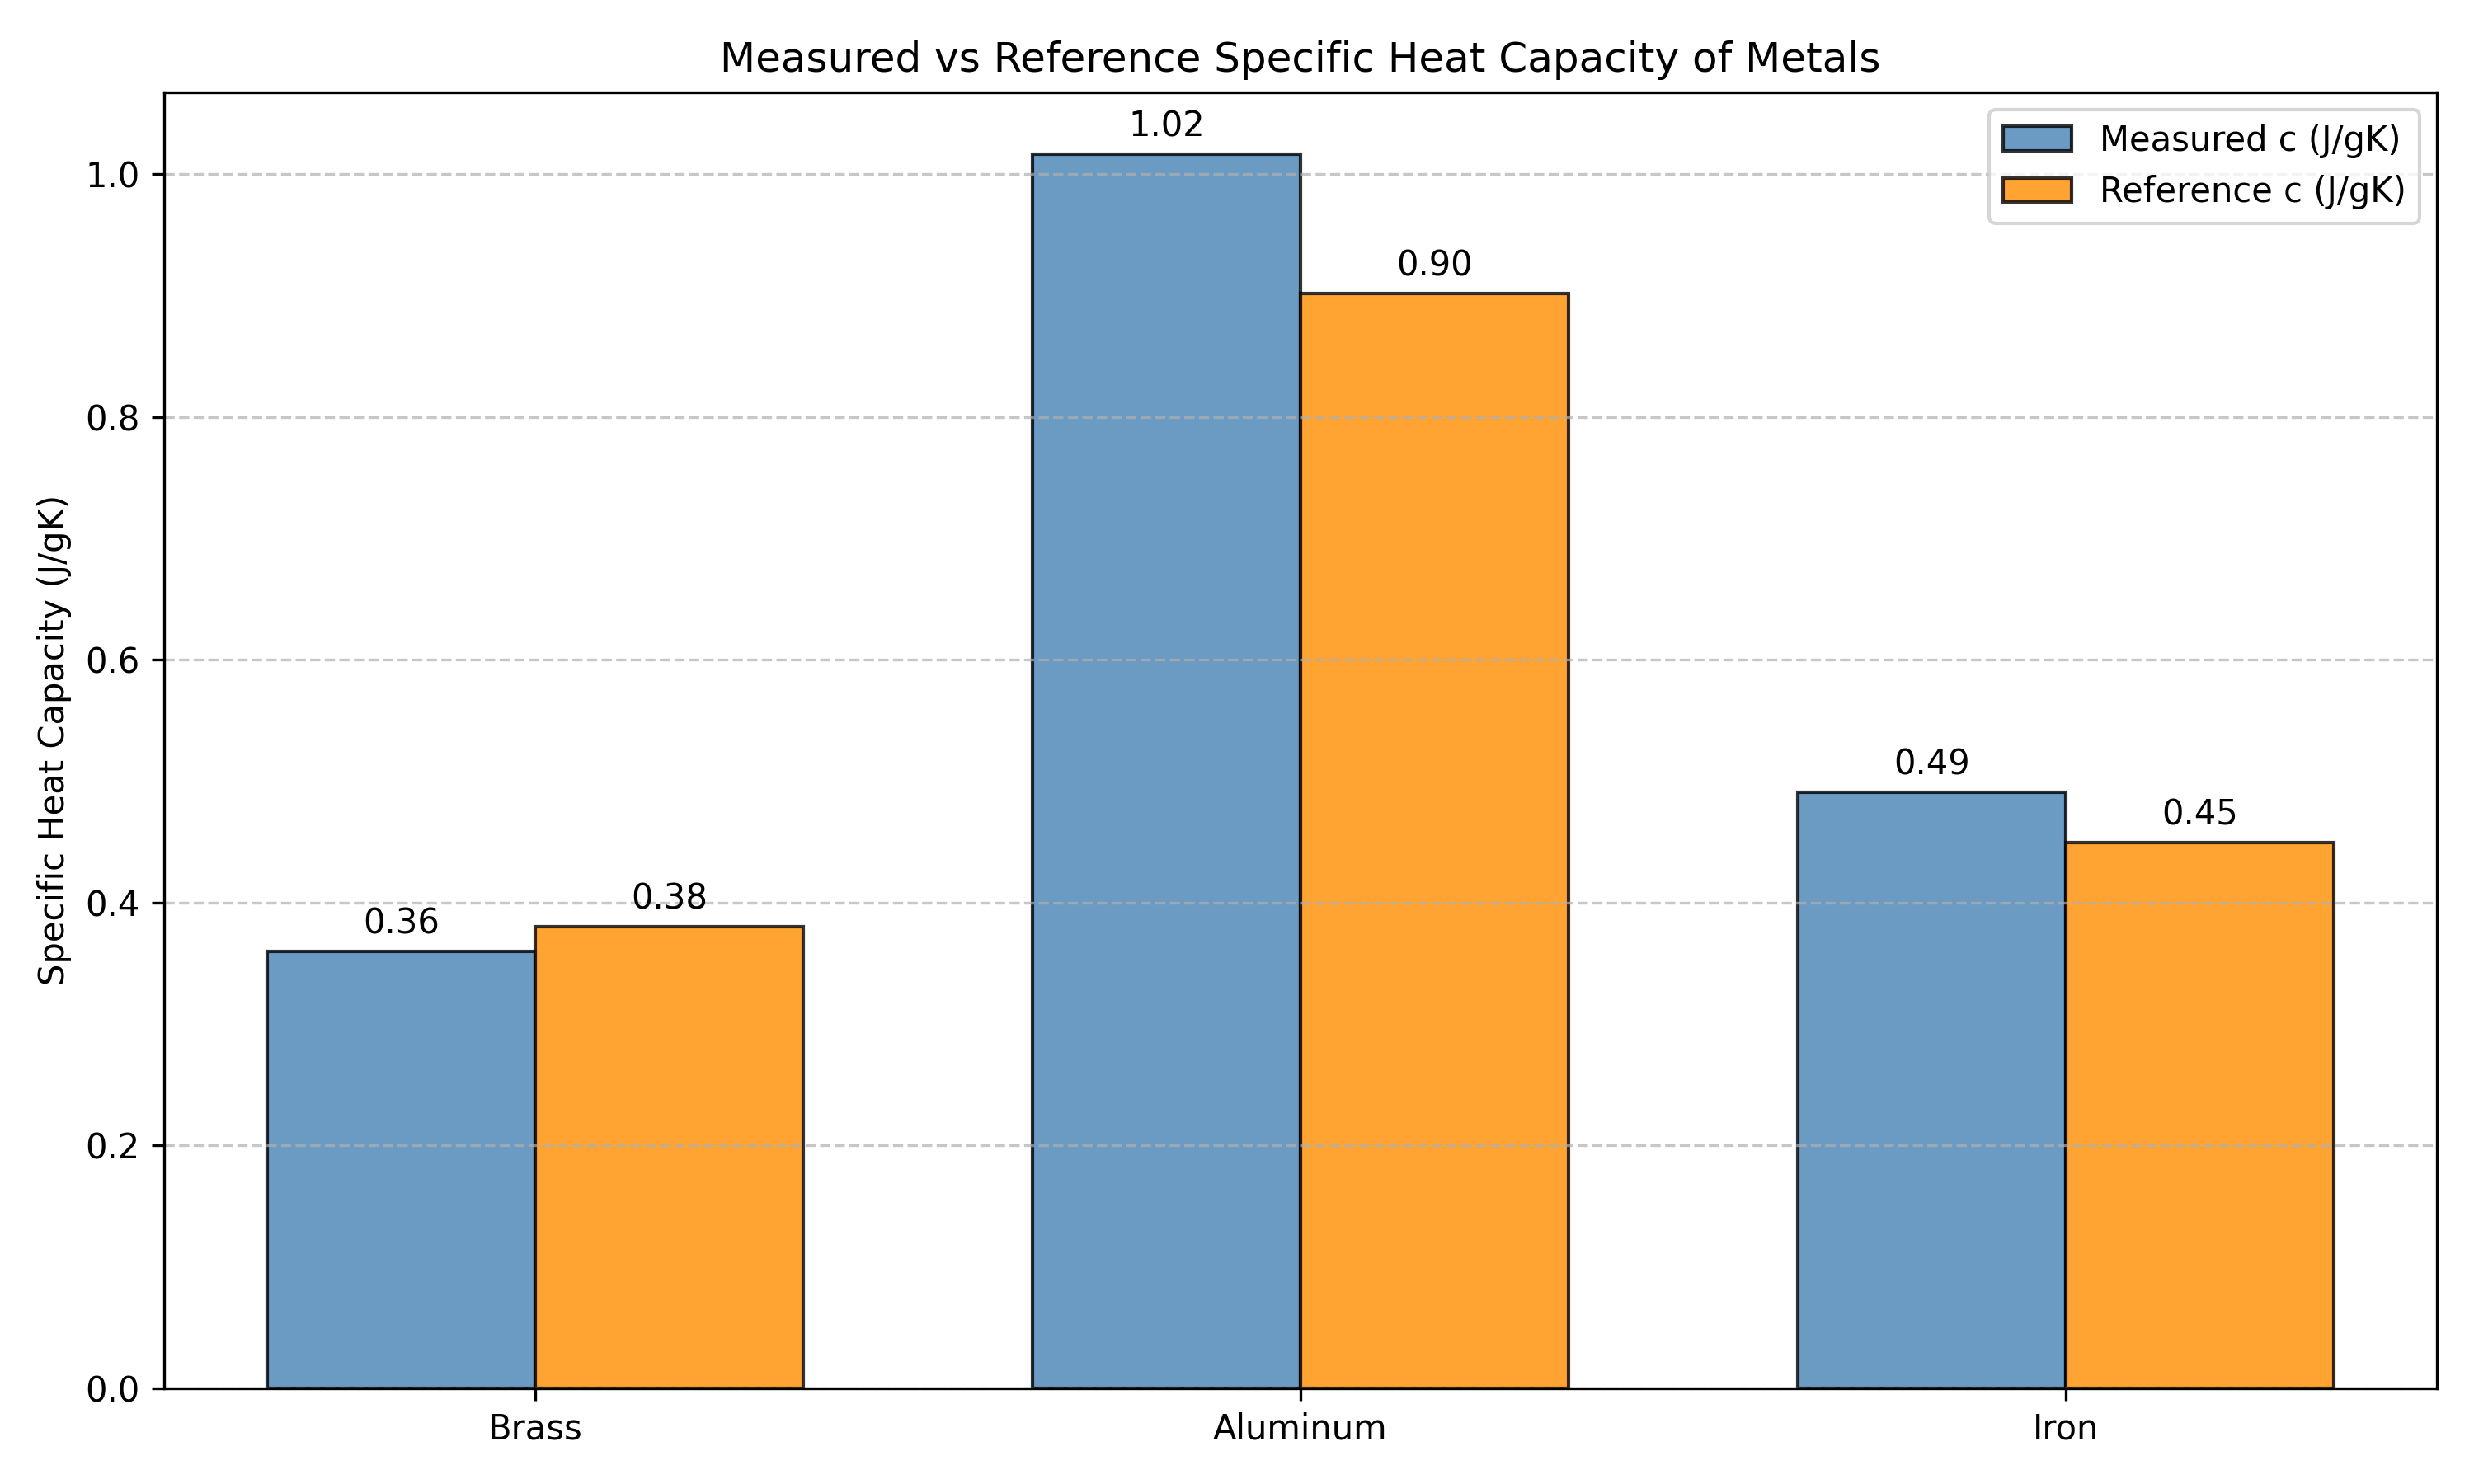
\includegraphics[width=\linewidth]{../plots/specific_heat_comparison.png}
    \caption{Comparison of measured specific heat capacities with reference values.}
    \label{fig:comparison}
\end{figure}

\newpage
% ---------- DISCUSSION ----------
\section{Discussion}
The results obtained for the specific heat capacities are reasonably close to the literature values, with percentage errors ranging from 5.4\% (Brass) to 12.7\% (Aluminum). 

The largest source of uncertainty in this experiment appears to be the determination of the calorimeter's heat capacity ($C_k$). The three trials for $C_k$ yielded widely divergent values ($1046$, $57$, and $342$ \si{J/K}), leading to a large standard deviation ($\approx \SI{509}{J/K}$). This suggests inconsistency in the calibration procedure, perhaps due to heat loss during the transfer of hot water or insufficient stabilization time.

All measured values were slightly higher (for Aluminum and Iron) or close (Brass) to the reference values. A higher measured specific heat might imply that the temperature change of the water ($\Delta T_{water}$) was smaller than expected for a given energy input, or that the system lost heat to the surroundings which was not accounted for. However, Equation \ref{eq:csample} shows that if $t_m$ is lower due to heat loss, $(t_m - t_k)$ decreases and $(t_2 - t_m)$ increases, which would generally lower the calculated $c$. The fact that we observe higher values for some metals might point to an overestimation of $C_k$, or that the mass of the water was slightly overestimated.

The formula used for $C_k$ (Eq. \ref{eq:Ck}) is also non-standard. If the standard energy balance had been used, the values for $C_k$ might have been different, significantly affecting the final results.


% ---------- CONCLUSION ----------
\section{Conclusion}
The specific heat capacities of Brass, Aluminum, and Iron were determined using the method of mixtures. The experimental values were \SI{0.360}{J/gK}, \SI{1.017}{J/gK}, and \SI{0.491}{J/gK} respectively. While the results confirm the material dependence of specific heat, the high uncertainty in the calorimeter constant highlights the importance of precise thermal isolation and consistent procedural timing in thermodynamic experiments.

% ---------- RESOURCES ----------
\section{Additional Resources}
For more information, scanned data, and the code used for analysis, refer to the repository:

\vspace{0.5em}
\noindent
\url{https://github.com/ibrahim-hamed/Physics-Lab}

\vspace{1em}
\begin{center}
    \qrcode[height=1in]{https://github.com/ibrahim-hamed/Physics-Lab}
\end{center}

% ---------- BIBLIOGRAPHY ----------
\begin{thebibliography}{9}
    \bibitem{manual}
    \emph{Experiment 2: Heat Capacity of Metals}, Laboratory Manual, Department of Physics, Istanbul University.
    
    \bibitem{greiner}
    W. Greiner, L. Neise, and H. Stöcker, \emph{Thermodynamics and Statistical Mechanics}, New York: Springer, 1995, p. 16.

    \bibitem{hyperphysics}
    R. Nave, ``Specific Heat,'' HyperPhysics, Georgia State University. [Online]. Available: \url{http://hyperphysics.phy-astr.gsu.edu/hbase/thermo/spht.html}

    \bibitem{engineeringtoolbox}
    Engineering ToolBox, ``Specific Heat of Metals,'' 2003. [Online]. Available: \url{https://www.engineeringtoolbox.com/specific-heat-metals-d_152.html}

    \bibitem{misumi}
    Misumi USA, ``Specific Heat Capacity of Metals,'' 2022. [Online]. Available: \url{https://us.misumi-ec.com/blog/specific-heat-capacity-of-metals/}

    \bibitem{libretexts}
    LibreTexts Chemistry, ``T4: Specific Heats and Molar Heat Capacities,'' 2020. [Online]. Available: \url{https://chem.libretexts.org/}
\end{thebibliography}

\end{document}
